\chapter{Modification apportée au programme de l'ESP32}

\section{Introduction}
Ce chapitre traite des modifications et amélioration apporté a l'interface web. La correction d'un chargement infini et l'ajout de la mesure du courant furent implémenter.

\section{Analyse de l'espace mémoire}
Le compilateur de l'environnement Arduino permet d'évaluer l'espace mémoire occupé au sein de l'ESP32. L'issue de la compilation fournit les informations suivantes concernant l'allocation mémoire :

\begin{quote}
  Le croquis utilise 979768 octets (74\,\%) de l'espace de stockage de programmes. Le maximum est de 1310720 octets.

  Les variables globales utilisent 45324 octets (13\,\%) de mémoire dynamique, ce qui laisse 282356 octets pour les variables locales. Le maximum est de 327680 octets.
\end{quote}

En ce qui concerne la taille des fichiers sources, le code propre à l'ESP32 représente 9,9~ko, tandis que celui définissant l'interface web occupe 10,6~ko.

La majorité de la mémoire est occupé principalement par les librairies lié au WIFI et du serveur web. Il a tout de meme été possible de réaliser les modifications apporté a l'ESP32.

\section{Modifications et correction sur la page web et la communication}
La page web actuel, permettais depuis le travail de bachelor précédent d'afficher des tracés de la positions. Cependant des problèmes de connections a l'interface WEB subsiste.

Une volonté d'afficher le courant fut désirer ce qui fut dès lors implémenter.

\subsection{Correction du chargement infinie}
Lors de la connexion a l'interface utilisateur, il arrivait que celle-ci présente un chargement infini.

Suite a des recherches, la raison fut trouver dans les fonctions de réponse du serveur, s'appelant \texttt{server.send()}. La réponse renvoyaies initialement le code 250. En se basant sur les références de statut conseiller pour le HTTP \cite{HTTPStatut}, celle-ci n'est pas un standard employer pour indiquer un succès d'une page web. La page WEB ne sait donc pas comment interpreter cette valeur et il arrive qu'elle l'accepte ou non. Dès lors elle fut changer par une valeur mieux connue des serveurs web étant la valeur de 200 qui indique un simple \texttt{OK}.

\subsection{Ajout de la mesure du courant}
Suite a la demande de Monsieur Girardin, la mesure de courant fut ajouter sur l'interface WEB.

Pour commencer il fallu modifier la fonction SendFloatAsText afin qu'elle puisse accepter 8 valeurs. Tout d'abord il est néscessaire de modifier la taille du buffer de la transmission \texttt{TX\_BUF\_LEN} en la modifiant de 64 à 128. Il faut ajouter également 4 nouvelle variable  dans les parenthèses de la fonction \texttt{SendFloatAsText}. Les modifications donne dès lors :

\begin{minted}{c}
#define TX_BUF_LEN 128
...
void SendFloatAsText(float f0, float f1, float f2, float f3, float f4, float f5, float f6, float f7)
{
    char str[TX_BUF_LEN];
    int i = 0, j = 0;

    str[i++] = '\x02'; // start bit

    i += ftoa(f0, &str[i], 3); str[i++] = ',';
    i += ftoa(f1, &str[i], 3); str[i++] = ',';
    i += ftoa(f2, &str[i], 3); str[i++] = ',';
    i += ftoa(f3, &str[i], 3); str[i++] = ',';
    i += ftoa(f4, &str[i], 3); str[i++] = ',';
    i += ftoa(f5, &str[i], 3); str[i++] = ',';
    i += ftoa(f6, &str[i], 3); str[i++] = ',';
    i += ftoa(f7, &str[i], 3);

    str[i++] = '\x03'; // stop bit

    for (j = 0; j < i && j < TX_BUF_LEN; j++) {
        txBuffer[j] = (uint8_t)str[j];
    }
    txLength = i;
    txIndex = 0;

    SCI_enableInterrupt(SCIA_BASE, SCI_INT_TXFF);
}
\end{minted}

Il faut également modifier le code du côté de l'ESP32 afin qu'il puisse accepter plus de valeurs.

Tout d'abbord, il faut augmenter la taille du buffer dédié a la ocmmunciation UART. Ceci se réalise en changeant la constante \texttt{UART\_BUFFER} de 64 à 128.

Ensuite, lorsque la trame est entièrement reçu, il faut augmenter la valeur max de la boucle \texttt{while(...)} gérant la conversion des données à 8.

Pour terminer, il faut que l'interface WEB puisse trouver les valeurs de courants. Des nouvelles balises XML furent dès lors créer afin d'indiquer a l'interface WEB les valeurs du courants. Celle-ci sont déclaré comme \texttt{<curIndX>} ou X représente un numéro allant de 1 à 4 selon l'inducteur.

Ceci donne alors les codes suivants :

\begin{minted}{cpp}
  #define UART_BUFFER 128
  ...
    // Traitement des données une fois toute la trame reçue
  if (RxIndex > 0) {
    // Ajout d'un caractère de fin
    buffer[RxIndex] = '\0';

    // Vérification de la forme de la trame
    if (buffer[0] == 0x02 && buffer[RxIndex - 1] == 0x03) {
      char* token = strtok(&buffer[1], ",");  // Découpe la chaîne après '\x02' et avant la première virgule de séparation
      int i = 0;

      // Conversion des token en floats
      while (token != NULL && i < 8) {
      floatValues[i++] = atof(token);
      token = strtok(NULL, ",");
      }

      // Afficher les floats reçus (facultatif)
      // Serial.print("Valeurs reçues : ");
      // for (int i = 0; i < 4; i++) {
      //   Serial.print(floatValues[i]);
      //   Serial.print(" ");
      // }
      // Serial.println();

      // Mise à jour des valeurs de position pour la page web
      updateValues();

      // Réinitialiser l'index du buffer après traitement
      RxIndex = 0;
    }
    // Si la trame ne commence pas par \x02 ou ne se termine pas par \x03, ignorer
    else {
      Serial.println("Trame invalide");
      RxIndex = 0;
    }
  }
  ...
    // send the inductor currents
  sprintf(buf, "<curInd1>%f</curInd1>\n", cur_ind1);
  strcat(XML, buf);
  sprintf(buf, "<curInd2>%f</curInd2>\n", cur_ind2);
  strcat(XML, buf);
  sprintf(buf, "<curInd3>%f</curInd3>\n", cur_ind3);
  strcat(XML, buf);
  sprintf(buf, "<curInd4>%f</curInd4>\n", cur_ind4);
  strcat(XML, buf);
\end{minted}

\noindent
\begin{minipage}[c]{0.55\textwidth}

  Le résultat est présent s
\end{minipage}%
\hfill
\begin{minipage}[c]{0.4\textwidth}
  \centering
  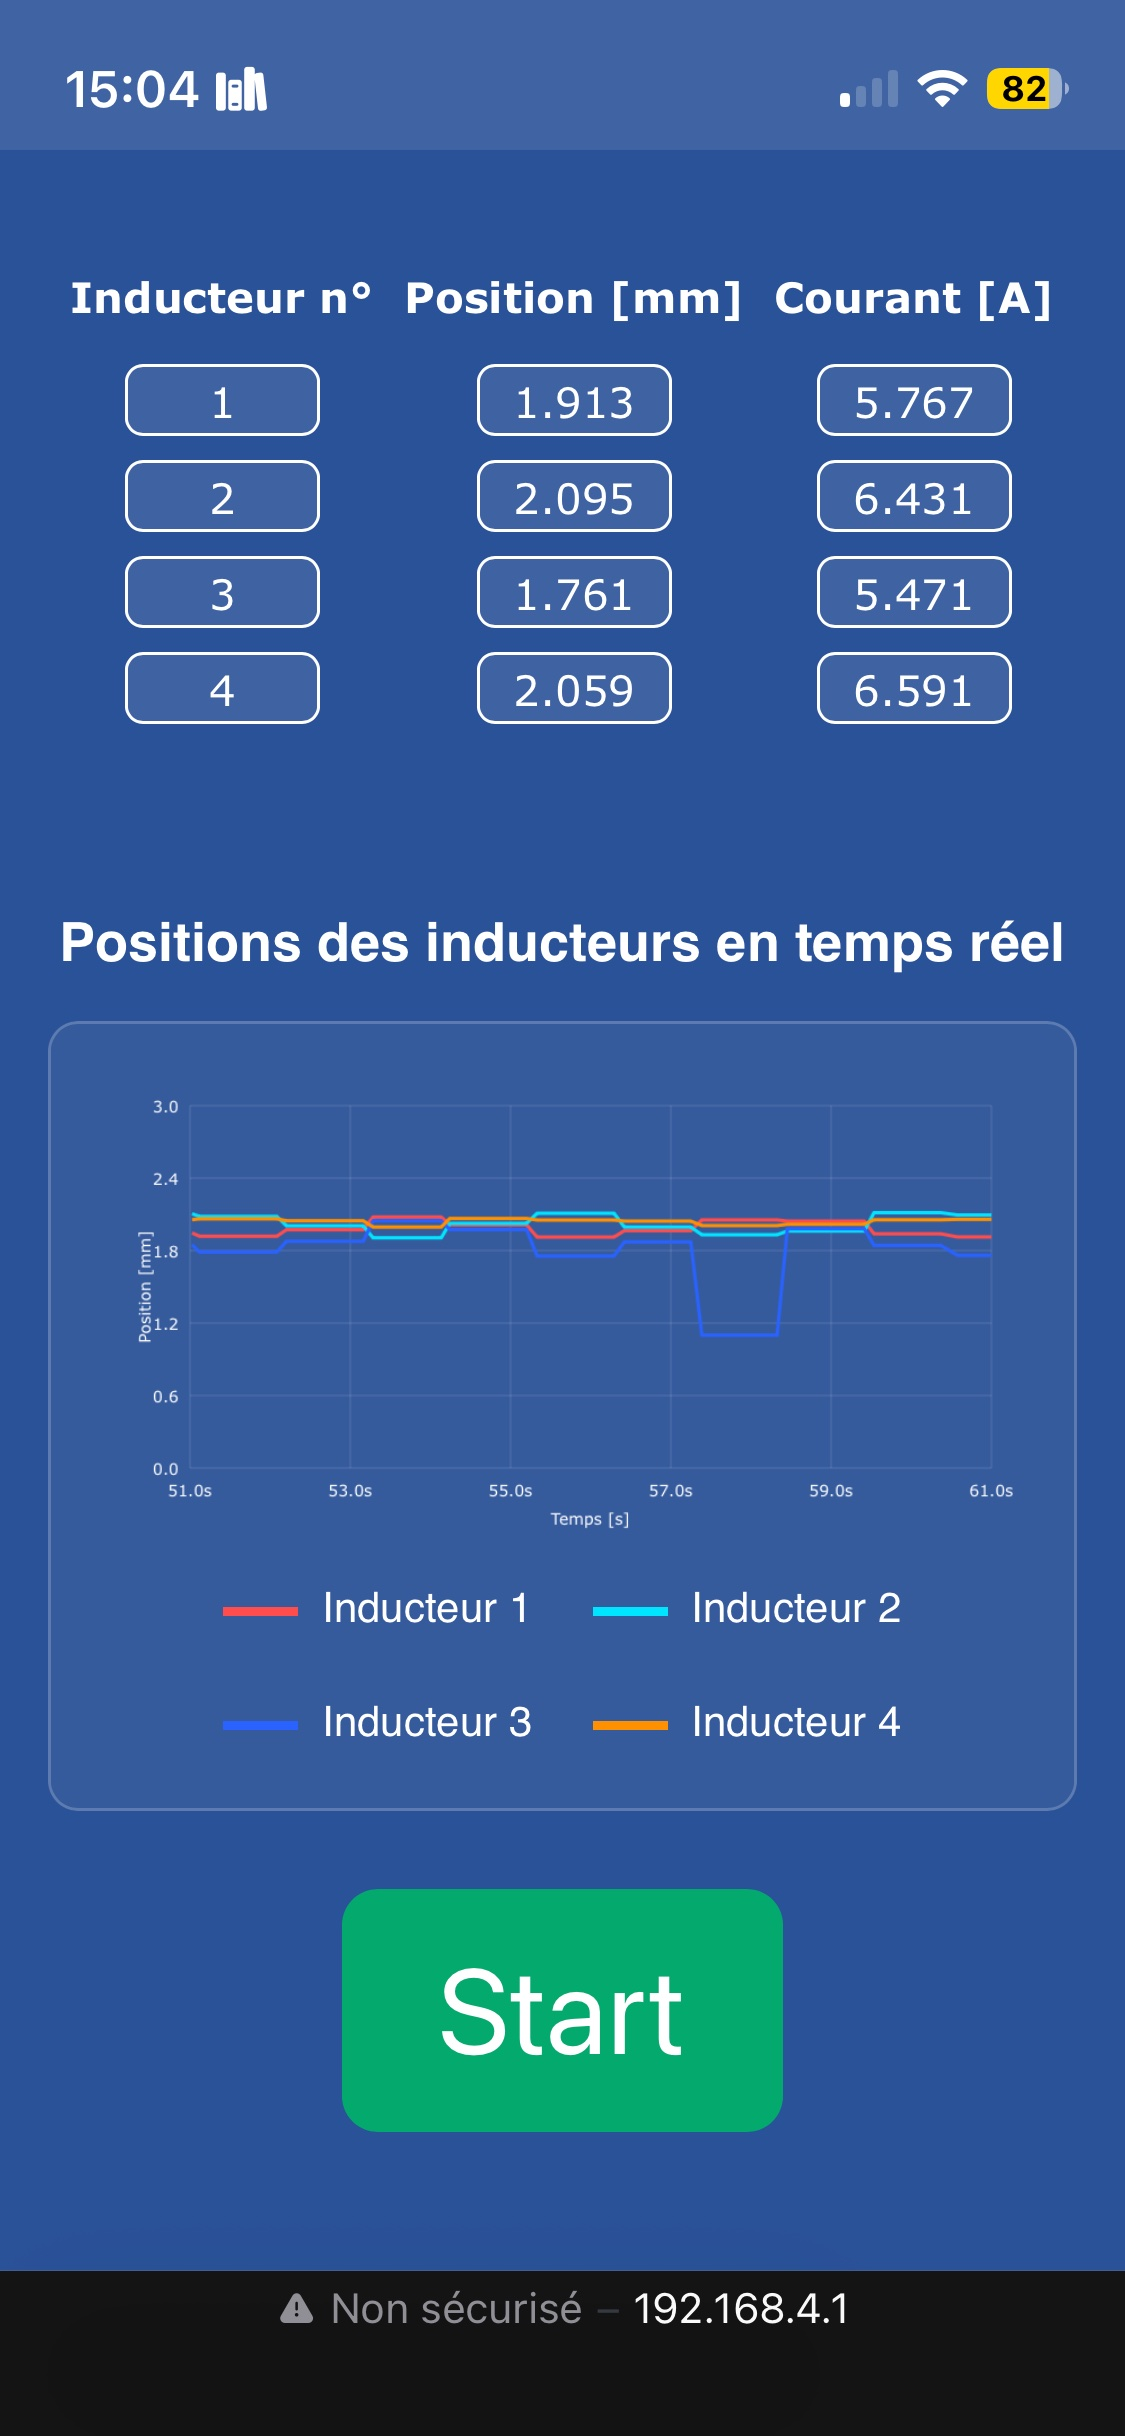
\includegraphics[trim = 0 10cm 0 8cm, clip, width=\linewidth]{assets/content/10-ModificationESP/InterfaceWeb.jpeg}
  \captionof{figure}{Interface WEB avec l'ajout du courant}
\end{minipage}

Pour commencer, il fallu ajouter une troisième collones sur l'interface web. Cette nouvelle colonnes est dédiée a l'affichage du courant. La valeur du courant est dès lors récupérer via la balise XML placer précédement dans le code arduino :

\begin{minted}{html}
<div class="inducteurs-colonnes">
  <div class="bloc-colonne">
    <div class="entete">Data</div>
    <div class="valeur" style="border:none; font-weight:bold;">Pos 1</div>
    <div class="valeur" style="border:none; font-weight:bold;">Pos 2</div>
    <div class="valeur" style="border:none; font-weight:bold;">Pos 3</div>
    <div class="valeur" style="border:none; font-weight:bold;">Pos 4</div>
  </div>
  <div class="bloc-colonne">
    <div class="entete">Position [mm]</div>
    <div class="valeur" id="valInd1">0.000</div>
    <div class="valeur" id="valInd2">0.000</div>
    <div class="valeur" id="valInd3">0.000</div>
    <div class="valeur" id="valInd4">0.000</div>
  </div>
  // Nouvelle colonne pour le courant
  <div class="bloc-colonne">
    <div class="entete">Courant [A]</div>
    <div class="valeur" id="curInd1">0.000</div>
    <div class="valeur" id="curInd2">0.000</div>
    <div class="valeur" id="curInd3">0.000</div>
    <div class="valeur" id="curInd4">0.000</div>
  </div>
</div>
  ...
  // Extraction des 8 valeurs (Pos 1..4 et Cur 1..4)
  var v_p1 = extractVal("valInd1");
  var v_p2 = extractVal("valInd2");
  var v_p3 = extractVal("valInd3");
  var v_p4 = extractVal("valInd4");

  var v_c1 = extractVal("curInd1");
  var v_c2 = extractVal("curInd2");
  var v_c3 = extractVal("curInd3");
  var v_c4 = extractVal("curInd4");

  // Mise à jour de l'affichage HTML
  document.getElementById("valInd1").innerHTML = v_p1.toFixed(3);
  document.getElementById("valInd2").innerHTML = v_p2.toFixed(3);
  document.getElementById("valInd3").innerHTML = v_p3.toFixed(3);
  document.getElementById("valInd4").innerHTML = v_p4.toFixed(3);

  document.getElementById("curInd1").innerHTML = v_c1.toFixed(3);
  document.getElementById("curInd2").innerHTML = v_c2.toFixed(3);
  document.getElementById("curInd3").innerHTML = v_c3.toFixed(3);
  document.getElementById("curInd4").innerHTML = v_c4.toFixed(3);
\end{minted}

L'interface fut également modifiée pour avoir une taille variable selon la taille de l'écran. Tout d'abord celle-ci vérifie la taille actuelle de l'écran. Si celle-ci est inférieur a 600px, alors l'interface pass a un affichage plus petit. De plus si l'écran s'avère réellement trop petite alors le principe d'un flex-warp est employé. Celui-ci vient tout simplement réaliser un retour  a la ligne du texte dans les collones. Cela est alors réalisé comme suit :

\begin{minted}{html}
  <meta name="viewport" content="width=device-width, initial-scale=1.0">
  ...
  /* Responsive (Téléphone) */
  @media (max-width: 600px) {
    .inducteurs-colonnes { gap: 15px; }
    .entete { font-size: 14px; }
    .valeur { font-size: 14px; width: 50px; padding: 4px; }
    .button { font-size: 24px; padding: 10px 20px; }
  }
\end{minted}

\subsection{Filtrage des données}
Les données affiché changeant très rapidement et régulirèmenet, des valeurs filtrés furent dès lors envoyer. Ceci fut réaliser via un filtre d'ordre 1 Cela se fait très simplement au niveau du programme principale comme suit :

\begin{minted}{c}
  Pos1_filt = (0.001 * Position1) + (0.999 * Pos1_filt);
  Pos2_filt = (0.001 * Position2) + (0.999 * Pos2_filt);
  Pos3_filt = (0.001 * Position3) + (0.999 * Pos3_filt);
  Pos4_filt = (0.001 * Position4) + (0.999 * Pos4_filt);

  Cur1_filt = (0.0001f * Current1) + (0.9999f * Cur1_filt);
  Cur2_filt = (0.0001f * Current2) + (0.9999f * Cur2_filt);
  Cur3_filt = (0.0001f * Current3) + (0.9999f * Cur3_filt);
  Cur4_filt = (0.0001f * Current4) + (0.9999f * Cur4_filt);
\end{minted}

Ceux-ci sont dès lors employé pour l'envoie des données :

\begin{minted}{c}
  UartCounter++;
  if (UartCounter >= 250)
  {
      UartCounter = 0;

      SendFloatAsText(Pos1_filt*1000, Pos2_filt*1000, Pos3_filt*1000, Pos4_filt*1000, Cur1_filt, Cur2_filt, Cur3_filt, Cur4_filt);
  }
\end{minted}